\begin{frame}[t]{Metamateriais}
    \transboxout[duration=0.5]
    \begin{columns}
        \column{.1\textwidth}
        \column{.4\textwidth}
            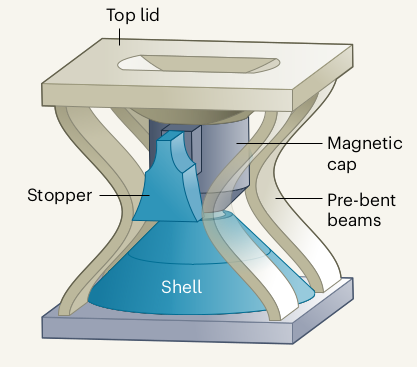
\includegraphics[width=.87\textwidth]{shell.png}
        \column{.6\textwidth}
            \begin{itemize}
                \item Formado por sub-unidades projetadas
                \item Propriedade não encontradas em materiais naturais
            
            \end{itemize}
    \end{columns}
    
    \note[item]{O objeto de estudo é um exemplo de metamaterial.}
\end{frame}